\documentclass{beamer}
%
% Choose how your presentation looks.
%
% For more themes, color themes and font themes, see:
% http://deic.uab.es/~iblanes/beamer_gallery/index_by_theme.html
%
\mode<presentation>
{
  \usetheme{Szeged}      % or try Darmstadt, Madrid, Warsaw, ...
  \usecolortheme{beaver} % or try albatross, beaver, crane, ...
  \usefonttheme{professionalfonts}  % or try serif, structurebold, ...
  \setbeamertemplate{navigation symbols}{}
  \setbeamertemplate{caption}[numbered]
} 

\usepackage[english]{babel}
\usepackage[utf8x]{inputenc}
\usepackage{graphicx}
\usepackage{svg}
\usepackage{amsmath}
\usepackage{booktabs}
\usepackage{algorithm}
\usepackage{algpseudocode}
\usepackage{hyperref}
\usepackage{tikz}
\usetikzlibrary{positioning,angles,quotes}
\usetikzlibrary{arrows,shapes}
\usepackage{caption}
\usepackage{media9}

\everymath{\displaystyle}
\DeclareMathOperator*{\argmin}{arg\,min}
\DeclareMathOperator*{\argmax}{arg\,max}

\title[Data efficient reinforcement learning]{Data efficient reinforcement learning\\Gaussian process, PILCO and DeepPILCO}
\author{Ali Younes}
\institute[BMSTU]
{
  Bauman Moscow State Technical University \\ % Your institution for the title page
  \medskip
  \textit{ay20-5-1994@hotmail.com} % Your email address
}
\date{\today}

\begin{document}

\begin{frame}
  \titlepage
\end{frame}

% Uncomment these lines for an automatically generated outline.
\begin{frame}{Outline}
  \tableofcontents
\end{frame}

\section{Introduction}
\subsection{Data efficient reinforcement learning}
\begin{frame}{Why data efficient reinforcement learning?}
\begin{itemize}
  \item Reinforcement learning is a hot research topic nowadays.\\
  It is considered one of the major research directions in robot learning.
  \item We have worked with model free algorithms (TRPO, PPO).
\end{itemize}
  \begin{center}
  \captionsetup{labelformat=empty}
  \captionof{figure}{Reinforcement learning}
    \tikzstyle{block} = [rectangle, draw, 
    text width=7em, text centered, rounded corners, minimum height=3em]
    \tikzstyle{line} = [draw, -latex]
    \begin{tikzpicture}[node distance = 6em, auto, thick]
        \node [block] (Agent) {Agent};
        \node [block, below of=Agent] (Environment) {Environment};
        \path [line] (Agent.0) --++ (4em,0em) |- node [near start,align=center]{Action \\ $a_t$} (Environment.0);
        \path [line] (Environment.180) --++ (-4em,0em) |- node [near start,align=center] {State \\ $s_{t+1}$ \\Reward \\$r_{t+1}$} (Agent.180);
    \end{tikzpicture}
\end{center}{}
\end{frame}

\begin{frame}
  \frametitle{Why data efficient reinforcement learning?}
  \begin{figure}[h]
      \centering
      \captionsetup{labelformat=empty}
      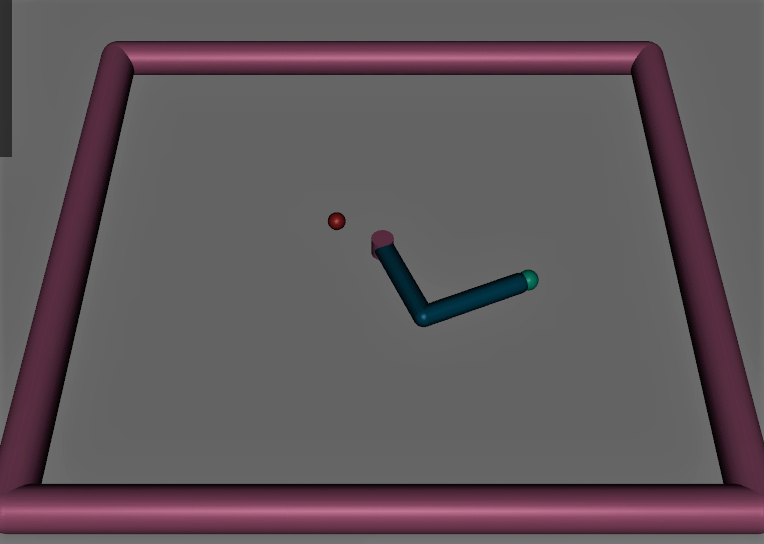
\includegraphics[height=6cm]{img/Reacher(Mujoco).png}
      \label{fig:my_label}
  \end{figure}
\end{frame}

\begin{frame}
  \frametitle{Why data efficient reinforcement learning?}
  \begin{figure}[h]
      \centering
      \captionsetup{labelformat=empty}
      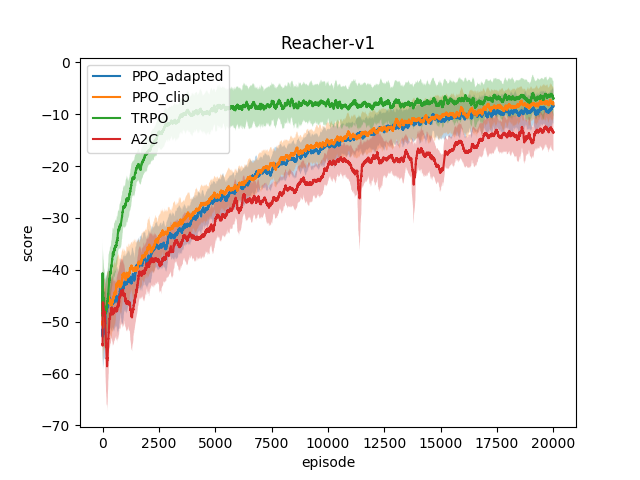
\includegraphics[height=7cm]{img/Reacher.png}
      \label{fig:my_label}
  \end{figure}
\end{frame}



\begin{frame}{Why data efficient reinforcement learning?}
\begin{itemize}
    \item In real world that means weeks of training.\\
    \textcolor{red}{Collecting samples is expensive in real world robots}
    \item We need a robot learning framework with as less as possible interaction time in the real world.\\
    Two solution:
    \begin{enumerate}
        \item Transfer learning from simulation to real world (Sim2Real)
        \item Data efficient learning
    \end{enumerate}
\end{itemize}
\end{frame}

\subsection{Gaussian Processes in RL}
\begin{frame}
  \frametitle{Model Based reinforcement learning}
\begin{center}
 \captionsetup{labelformat=empty}
 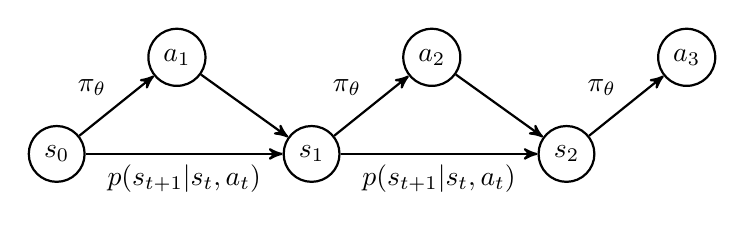
\begin{tikzpicture}[->, >=stealth', auto, thick, node distance=3cm]

    \tikzstyle{round}=[thick,draw=black,circle]

    \node[round] (s0) {$s_0$};
    \node[round,right= 25mm of s0] (s1) {$s_1$};
    \node[round,above right=7mm and 10mm of s0] (a1){$a_1$};
    \node[round,right= 25mm of s1] (s2) {$s_2$};
    \node[round,above right=7mm and 10mm of s1] (a2){$a_2$};
    \node[round,above right=7mm and 10mm of s2] (a3){$a_3$};

    \path (s0) edge node[below] {$p(s_{t+1}|s_t,a_t)$}(s1)
          (s0) edge node {$\pi_\theta$} (a1)
          (a1) edge node {} (s1);
    \path (s1) edge node[below] {$p(s_{t+1}|s_t,a_t)$}(s2)
          (s1) edge node {$\pi_\theta$} (a2)
          (a2) edge node {} (s2);
    \path (s2) edge node {$\pi_\theta$} (a3);
\end{tikzpicture}
\end{center}
\begin{itemize}
    \item We will use the following terminology:\\
    State : $x_t$ , Control (action): $u_t$ , Cost (reward): $c$
    \item Transition function: $x_{t+1}=f(x,u_t)+\omega$
    \item Control: $u_t=\pi (x_t,\theta )$
    \item The expected long-term cost:  $J(\theta)=\sum_{t=1}^{T} \mathbb{E} [c(x_t)|\theta]$
\end{itemize}
\end{frame}

\begin{frame}
	\frametitle{Gaussian processes}
    \begin{itemize}
    \item In probability theory and statistics, a Gaussian process is a stochastic process (a collection of random variables indexed by time or space), such that every finite collection of those random variables has a multivariate normal distribution, i.e. every finite linear combination of them is normally distributed.
    \item In other words, a  Gaussian process is a probability distribution over possible functions.
    \item Gaussian process defined by:
    \begin{enumerate}
        \item Mean function $m(.)$
        \item Covariance function (Kernel) $k(.,.)$
    \end{enumerate}
    \end{itemize}
\end{frame}

\begin{frame}{Gaussian processes - Regression}
\begin{center}
    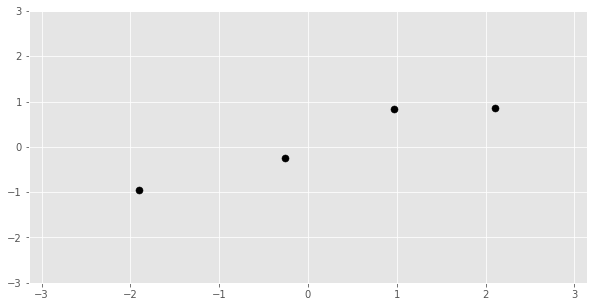
\includegraphics[height=3cm]{img/data.png}
    
    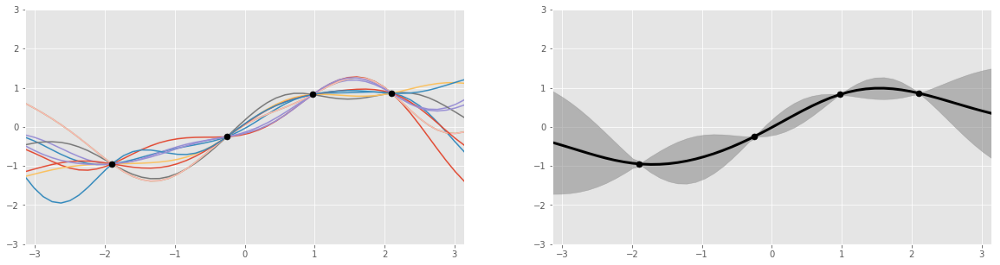
\includegraphics[height=3cm]{img/DPregression.png}
\end{center}
\end{frame}

\section{PILCO}

\subsection{PILCO Algorithm}

\begin{frame}
  \frametitle{PILCO Algorithm}
  \begin{itemize}
  \item Gaussian processes for data efficient learning in robotics and control\\
        (Marc Deisenroth, Dieter Fox, Carl Edward Rasmussen 2015)
  \item PILCO (Probabilistic Inference for Learning COntrol)
  \item A model based policy search method, considering the model uncertainty while learning models. PILCO Uses Gaussian processes as a probabilistic model.
  \end{itemize}
\end{frame}

\begin{frame}
\frametitle{PILCO Algorithm: High-level steps}
\begin{enumerate}
    \item Probabilistic model for transition function f \\
     (system identification)
    \item Compute long-term predictions $p(x_1|\theta),....,p(x_T|\theta)$
    \item Policy improvement
    \item Apply controller
\end{enumerate}
\end{frame}

\subsection{PILCO Algorithm components}
\begin{frame}{1. Model Learning (System Identification)}
    Model learning problem: Find a function $f:x \mapsto f(x)=y$
    \begin{center}
        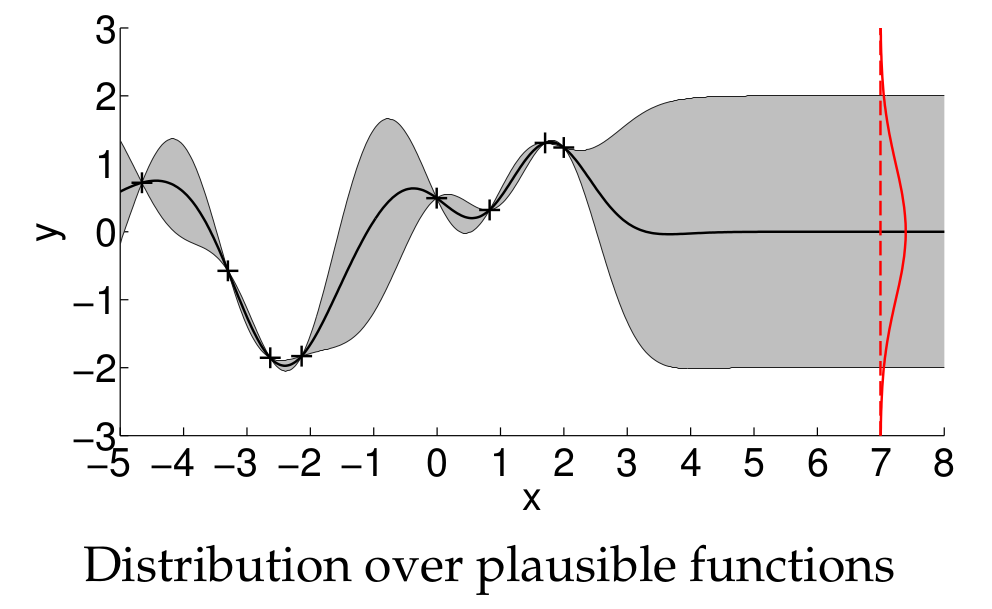
\includegraphics[height=4cm]{img/modellearning.png}
    \end{center}
    Express uncertainty about the underlying function to be robust to model errors. Posterior GP prediction $p(x_{t+1}|x_t,u_t)$
\end{frame}

\begin{frame}{2. Long-Term Predictions (Policy evaluation)}
    \begin{center}
        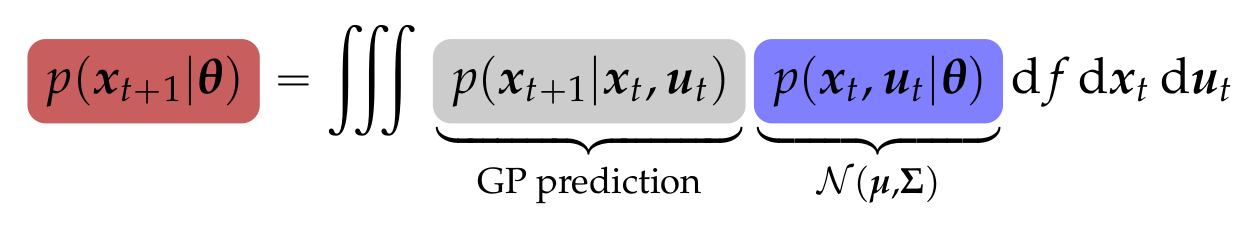
\includegraphics[height=1.8cm]{img/ltd-eq.png}\\
        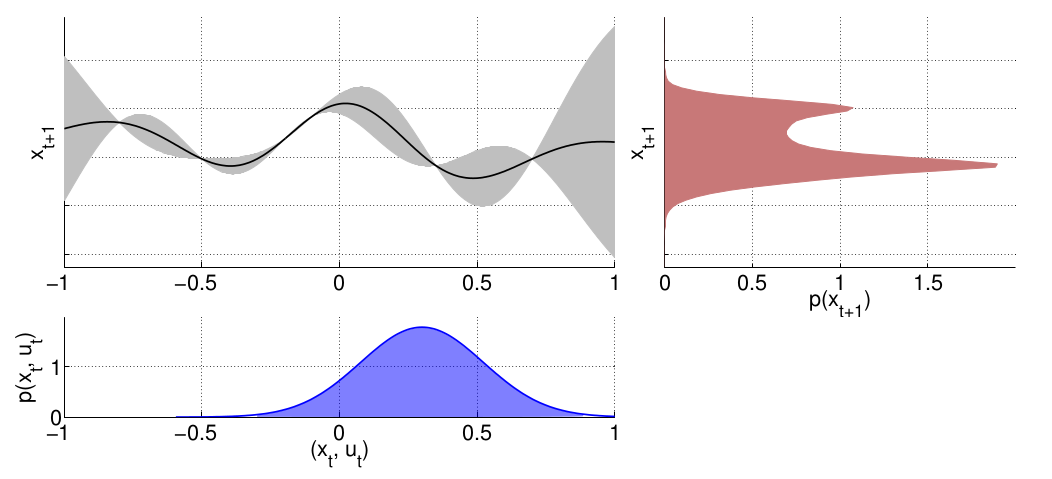
\includegraphics[height=5cm]{img/ltp.png}
    \end{center}
\end{frame}

\begin{frame}{2. Long-Term Predictions (Policy evaluation)}
Approximating $p(x_t+1)$ (red in the last image) by a Gaussian.\\
Using : 1. linearization of the posterior mean function
\begin{center}
    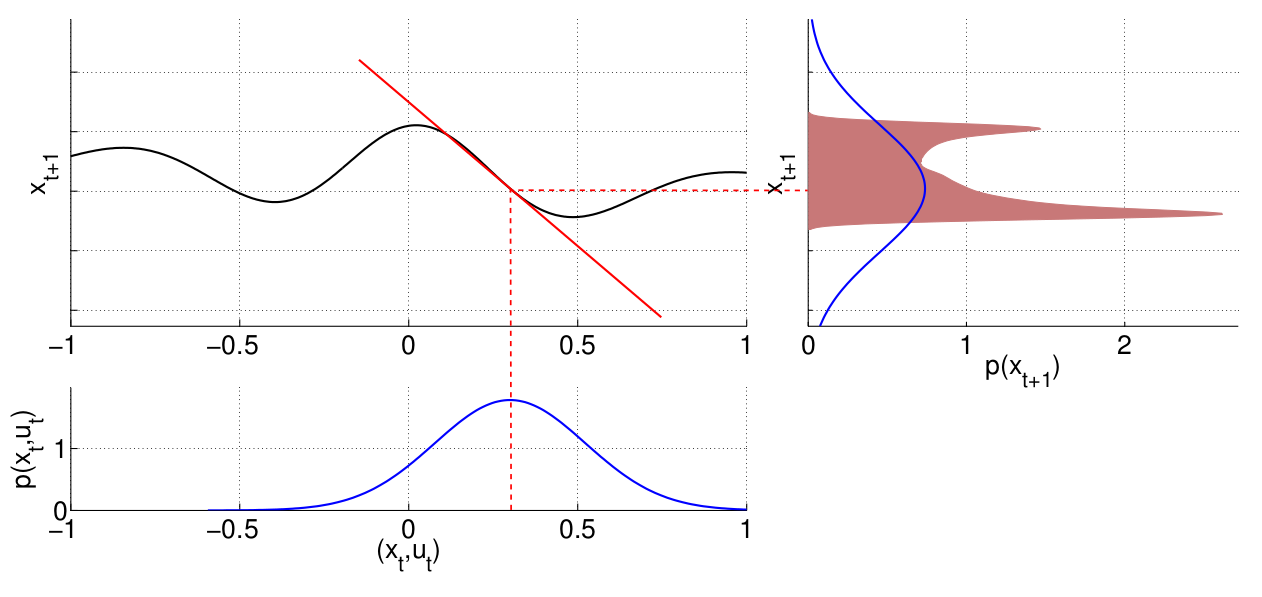
\includegraphics[height=5cm]{img/lin.png}
\end{center}
\end{frame}

\begin{frame}{2. Long-Term Predictions (Policy evaluation)}
Approximating $p(x_t+1)$ (red in the last image) by a Gaussian.\\
Using : 2. Moment matching
\begin{center}
    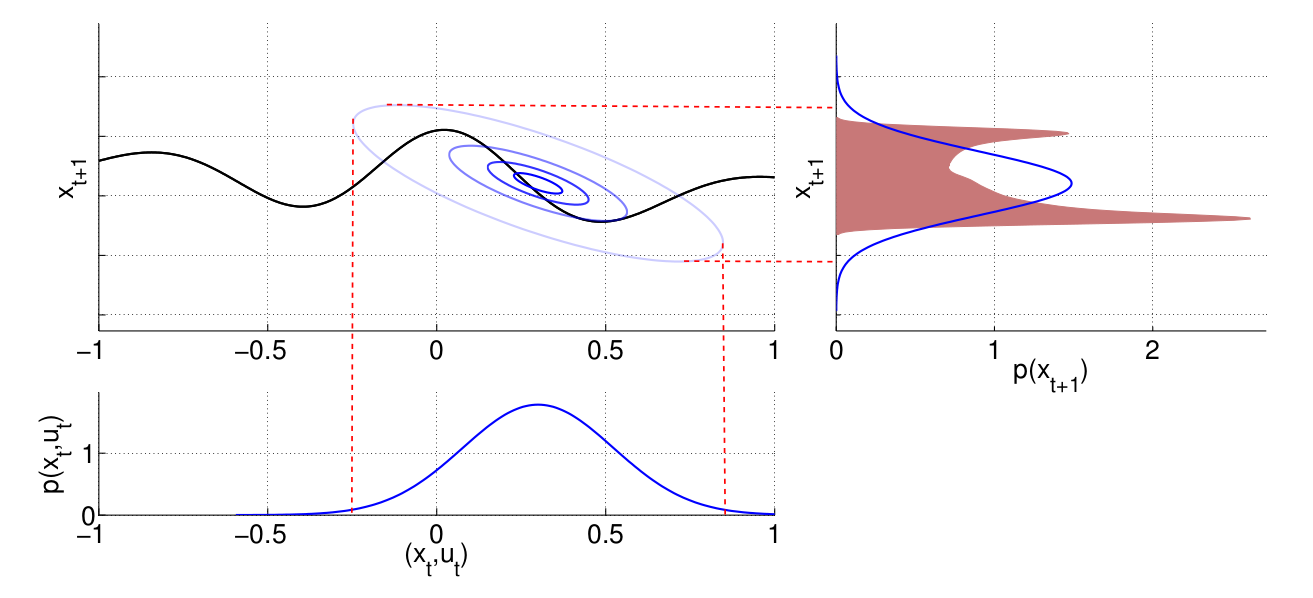
\includegraphics[height=5cm]{img/mom.png}
\end{center}
\end{frame}

\begin{frame}{2. Long-Term Predictions (Policy evaluation)}
To evaluate expected long term cost $J(\theta)$ we choose cost function $c$ such that inner the integral can be computed \textcolor{red}{analytically}:
$$J(\theta)=\sum_{t=1}^{T} \mathbb{E} [c(x_t)|\theta]=\sum_{t=1}^{T} \int c(x_t) \mathcal{N}(x_t|\mu_t,\Sigma_t) dx_t$$
\end{frame}

\begin{frame}{3. Policy Improvement and 4. Apply controller}
\begin{itemize}
    \item Analytically compute $\frac{d J^\pi (\theta)}{d\theta}$ for a gradient based policy search.
    \item We use standard gradient based optimizer (e.g. BFGS) to compute $\theta^*$
    \item Apply controller
\end{itemize}
\end{frame}

\subsection{Experimental results}
\begin{center}
Learning to Control a Low-Cost Manipulator
    \href{https://www.youtube.com/watch?v=gdT6dwUOYC0}{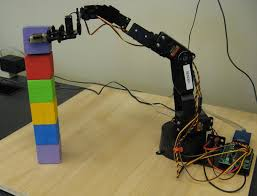
\includegraphics{img/arm.png}}
\end{center}

\section{Deep PILCO}
\subsection{PILCO problems}
\begin{frame}
  \Huge{\centerline{Thanks!}}
\end{frame}

\end{document}
